 \documentclass{beamer}
%
% Choose how your presentation looks.
% For more themes, color themes and font themes, see:
% http://deic.uab.es/~iblanes/beamer_gallery/index_by_theme.html
%
\mode<presentation>
{
  \usetheme{Madrid}      % or try Darmstadt, Madrid, Warsaw, ...
  \usecolortheme{seahorse} % or try albatross, beaver, crane, ...
  \usefonttheme{serif}  % or try serif, structurebold, ...
  \setbeamertemplate{navigation symbols}{}
  \setbeamertemplate{caption}[numbered]
  \setbeamertemplate{itemize/enumerate body begin}{\large}
\setbeamertemplate{itemize/enumerate subbody begin}{\large}
\setbeamertemplate{itemize/enumerate subsubbody begin}{\large}

  \usepackage{amsmath}
  \usepackage{bm}
  \usepackage{subcaption}
  \usepackage{tcolorbox}
  \usepackage[export]{adjustbox}
  \tcbuselibrary{most}
  \usepackage{arydshln}
  \usepackage{tikz}
  \usetikzlibrary{plotmarks}
  \usepackage{pgfplots}
  \usepackage{booktabs}
\usepackage[inkscapeformat=png]{svg}
 %\usepackage{enumitem}
%\usepackage{enumerate}
  %\usepackage[shortlabels]{enumitem}
} 


\definecolor{myblue}{RGB}{65,105,225} 
\definecolor{myorange}{RGB}{250,190,0}

\setbeamercolor{structure}{fg=white,bg=myorange}
\setbeamercolor*{palette primary}{fg=myblue,bg=myorange}
\setbeamercolor*{palette secondary}{fg=white,bg=myblue}
\setbeamercolor*{palette tertiary}{bg=myblue,fg=white}
\setbeamercolor*{palette quaternary}{fg=white,bg=myorange!50}

\setbeamercolor{frametitle}{fg=black!90!myblue}

\setbeamercolor{section in head/foot}{fg=white,bg=myblue}
\setbeamercolor{author in head/foot}{fg=black,bg=myorange}
\setbeamercolor{title in head/foot}{fg=white,bg=myblue}

\setbeamertemplate{navigation symbols}{}

\setbeamertemplate{itemize/enumerate body begin}{\large}
\setbeamertemplate{itemize/enumerate subbody begin}{\large}


\defbeamertemplate*{headline}{mytheme}
{%
  \begin{beamercolorbox}[ht=2.25ex,dp=3.75ex]{section in head/foot}
    \insertnavigation{\paperwidth}
  \end{beamercolorbox}%
}%

\defbeamertemplate*{footline}{mytheme}
{
  \leavevmode%
  \hbox{%
  \begin{beamercolorbox}[wd=.5\paperwidth,ht=2.25ex,dp=1ex,right]{author in head/foot}%
    \usebeamerfont{author in head/foot}\insertshortauthor\hspace*{2em}
  \end{beamercolorbox}%
  \begin{beamercolorbox}[wd=.5\paperwidth,ht=2.25ex,dp=1ex,left]{title in head/foot}%
    \usebeamerfont{title in head/foot}\hspace*{2em}\insertshortsubtitle\hspace*{2em}
    \insertframenumber{} / \inserttotalframenumber
  \end{beamercolorbox}}%
  \vskip0pt%
}


\usepackage[greek,german,russian,french,english]{babel}
\usepackage[LAE,T1]{fontenc}
%\usepackage[utf8x]{inputenc}
\usepackage{xcolor}
\usepackage{xurl}
\usepackage{listings}
\usepackage{pgf}  
\usepackage{textpos}
\usepackage{tabulary}
\usepackage{scrextend}
\usepackage{hyperref}
\usepackage{setspace}
\usepackage{rotating}
\lstset
{
    language=[LaTeX]TeX,
    breaklines=true,
    basicstyle=\tt\scriptsize,
    %commentstyle=\color{green}
    keywordstyle=\color{blue},
    %stringstyle=\color{black}
    identifierstyle=\color{magenta},
}
\newcommand{\bftt}[1]{\textbf{\texttt{#1}}}
%\newcommand{\comment}[1]{{\color[HTML]{008080}\textit{\textbf{\texttt{#1}}}}}
\newcommand{\cmd}[1]{{\color[HTML]{008000}\bftt{#1}}}
\newcommand{\bs}{\char`\\}
\newcommand{\cmdbs}[1]{\cmd{\bs#1}}
\newcommand{\lcb}{\char '173}
\newcommand{\rcb}{\char '175}
\newcommand{\cmdbegin}[1]{\cmdbs{begin\lcb}\bftt{#1}\cmd{\rcb}}
\newcommand{\cmdend}[1]{\cmdbs{end\lcb}\bftt{#1}\cmd{\rcb}}

\newcommand{\wllogo}{\textbf{Overleaf}}

% this is where the example source files are loaded from
% do not include a trailing slash
\newcommand{\fileuri}{https://raw.githubusercontent.com/GiancarloSucci/UniBo.IDSEPC.A2022/main/A2022.IDSEPCLaTeX/}


\usepackage{stackengine}
\def\Ruble{\stackengine{.67ex}{%
  \stackengine{.48ex}{\textsf{P}}{\rule{.8ex}{.12ex}\kern.6ex}{O}{r}{F}{F}{L}%
  }{\rule{.8ex}{.12ex}\kern.6ex}{O}{r}{F}{F}{L}\kern-.1ex}



%----------------------------------------------------------------------------------------
%	TITLE PAGE
%----------------------------------------------------------------------------------------
\title[L07]{Artificial Intelligence, Blockchain, e Criptovalute nello Sviluppo Software \newline\newline
Lezione 8: Change (in SW Development)} % The short title appears at the bottom of every slide, the full title is only on the title page

\author[{\tiny Giancarlo Succi }]{Giancarlo Succi\\\\ Dipartimento di Informatica -- Scienza e Ingegneria\\Universit\`{a} di Bologna\\
\bftt{g.succi@unibo.it}
} % Your name
\institute[unibo] % Your institution as it will appear on the bottom of every slide, may be shorthand to save space


\date{} % Date, can be changed to a custom date

\setbeamertemplate{navigation symbols}{}
\AtBeginSection[]
{
        \begin{frame}<beamer>{Outline}
                \tableofcontents[currentsection]
        \end{frame}
}
\begin{document}

\begin{frame}
\titlepage % Print the title page as the first slide

\end{frame}

%=============================================

\addtobeamertemplate{frametitle}{}{%
\begin{textblock*}{10mm}(-0.01mm,-0.95cm)

\includegraphics[width=0.9cm]{unibo-logo.png}
\end{textblock*}}

%=============================================


\begin{frame}
{\centerline{Structure of the lecture}}
\begin{itemize}
    \item Change (in Software Engineering)
    \item The experiment of Belyaev
    \item Understanding Change
    \end{itemize}
\end{frame}

\begin{frame}
{\centerline{Relevance of Change in Software Engineering}}
 
\begin{itemize}
\item Change is an overarching problem in software development given:
\begin{itemize}
\item the infancy of the discipline
\item the uncertainty of requirements
\item the constantly evolving technology
\item the intrinsic lock-ins
\end{itemize} 
\item However, while there are:
\begin{itemize}
\item technical approaches supporting change and
\item strong advocacies that change is essential
\end{itemize} 
still there is not an established approach to manage change into processes and people
\end{itemize} 

\end{frame}

\begin{frame}
{\centerline{Change Management in Software Engineering}}
 
\begin{itemize}
\item Preventing change \textcolor{red}{via detailed requirements}
\item Anticipating change via, for instance, \textcolor{red}{domain analysis} and variation points
\item Managing change, especially via maintenance
\begin{itemize}
\item \textcolor{red}{Corrective} maintenance
\item \textcolor{cyan}{Perfective} maintenance and \textcolor{red}{\textbf{refactoring}}
\item \textcolor{orange}{Adaptive} maintenance
\item \textcolor{blue}{Preventive} maintenance
\end{itemize} 
\end{itemize} 

\end{frame}




\begin{frame}
{\centerline{The concept of change in history (1/4)}}
 
\begin{itemize}
 \item From a anthropological perspective, changing is an important ability of the humankind
\begin{itemize}
\item  the ability to ``change'' has allowed us to survive and prosper for millenniums.
\end{itemize} 
\item Change has been part of the culture of the human kind
\begin{itemize}
\item the religion of the ancient Greece was nurtured by a constant change of the divinity and the humanity:
\begin{itemize}
\item see for instance the \foreignlanguage{greek}{μετεμψύχωσις} 
\item or the the Eraclitean statement \foreignlanguage{greek}{πάντα ῥεῖ}.
\end{itemize} 

\end{itemize} 

\end{itemize} 

\end{frame}

\begin{frame}
{\centerline{The concept of change in history (2/4)}}
\begin{itemize}
\item The same concept was present in the Roman culture, just think at the poet Ovid who wrote a poem about the always changing word, the Metamorphoses:
\end{itemize} 

\begin{center}
 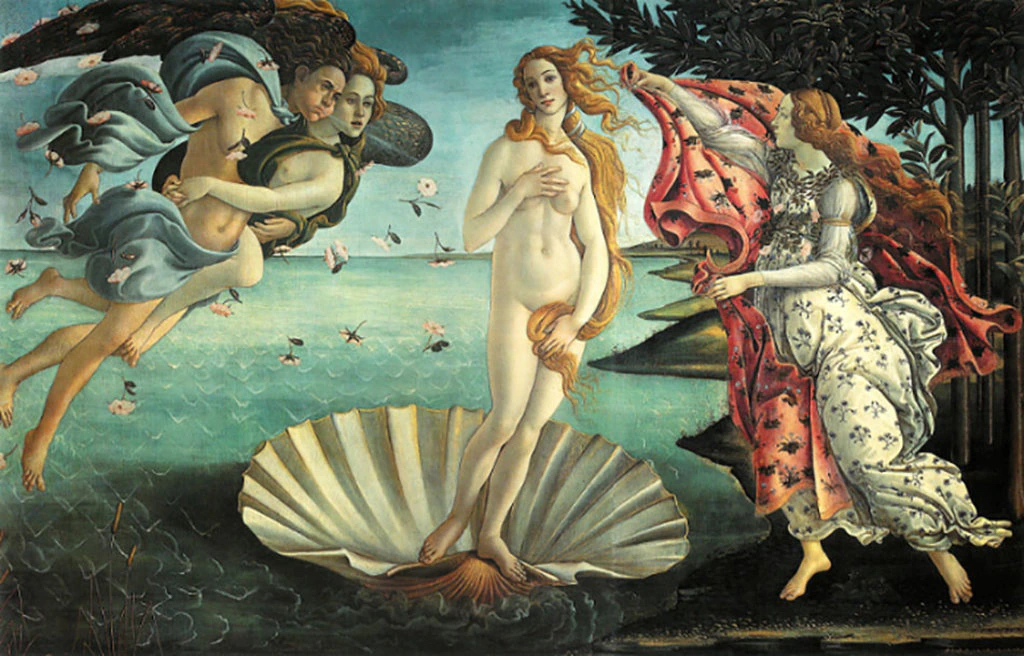
\includegraphics[width=8cm]{P2023.AIBCCSS.Change/LaNascitaDiVenere.jpg}
 
 \end{center}

\end{frame}

\begin{frame}
{\centerline{The concept of change in history (3/4)}}
 
\begin{itemize}
 \item Several Eastern religions are rooted in the concept of circularity and permanent change
 \item Still, change is also present in western religions:
\begin{itemize}
\item  Ebraism is rooted in change, as exemplified by the multiple ``Exodus''
\item  Christianity has as a center on the \foreignlanguage{greek}{μετάνοια} (``metanoia''), see St. Augustin
\item in Islam also the concept of  ``Tawbah'' \bgroup\fontencoding{LAE}\selectfont توبة\egroup ~ (``Tawbah'' ) plays an important role, together with repentance
\end{itemize} 
\end{itemize} 

\end{frame}

\begin{frame}
{\centerline{The concept of change in history (4/4)}}
 
\begin{itemize}
 \item Also several phylosophers have interpreted the human life as a constant change, whether circular of evolutionary
 \item In the middle age we could remember, among many:
 \begin{itemize}
 \item Gioacchino da Fiore (1135-1202) with, among other concepts, the theory of the \textcolor{red}{three ages}
\end{itemize} 
 \item and then among many others:
\begin{itemize}
\item Giovan Battista Vico (1668--1744) with the concept of the  \textcolor{red}{historical cycles}
\item  Friedrich Hegel (1770--1831) with the \textcolor{red}{phenomenology of spirit}
\item Karl  Marx (1818--1883) with the \textcolor{red}{dialectical materialism} (with Engels)
\item Friedrich Nietzsche (1844--1900) with the \textcolor{red}{eternal return}
\end{itemize} 
\end{itemize} 

\end{frame}

\begin{frame}
{\centerline{Change as a ``magic'' buzzword (1/6)}}
 
\begin{itemize}
 \item It has been often used interchangeably with  \textbf{\textcolor{red}{renewal}}.
 \item Using the positive connotation given to the term ``change,'' it has been used to pass \textit{negative} concepts, as a kind of anchoring:
 \begin{itemize}
\item This has well been explained by Schopenhauer in his essay on the art of being right, proposition 12
 \begin{itemize}
\item ``If the conversation turns upon some general conception which has no particular name, but requires some figurative or metaphorical designation, you must begin by choosing a metaphor that is favourable to your proposition. For instance, the names used to denote the two political parties in Spain, \textit{Serviles} and \textit{Liberales}, are obviously chosen by the latter. [$\ldots{}$]''
 \end{itemize} 
 \end{itemize} 
  \end{itemize} 
\begin{center}
\tiny
Source of the content: \url{http://coolhaus.de/art-of-controversy/erist12.htm}.
\end{center}

\end{frame}


\begin{frame}
{\centerline{Change as a ``magic'' buzzword (2/6)}}
 
\begin{itemize}
\item After Schopenhauer
 \begin{itemize}
\item This has been properly described in the blog of Sylvain Timsit 
 \begin{itemize}
\item ``Strategies of manipulations. [$\ldots{}$] 6. Appeal to the emotion rather than to the reflection. [$\ldots{}$]''
  \item Indeed, this takes advantage of the typical heuristics of the human mind
\end{itemize} 
\item Naom Chomsky has expressed a similar approach in his work, see for instance a collection of his essays: ``Language and Politics,'' edited by C. P. Otero
 \end{itemize} 
  \end{itemize} 
  
\begin{center}
\tiny
Source of the content: \url{http://www.syti.net/Manipulations.html}.
\end{center}



\end{frame}

\begin{frame}
{\centerline{Change as a ``magic'' buzzword (3/6)}}
 
\begin{itemize}
 \item Obama calls for renewal:
 \end{itemize} 
\begin{center}
 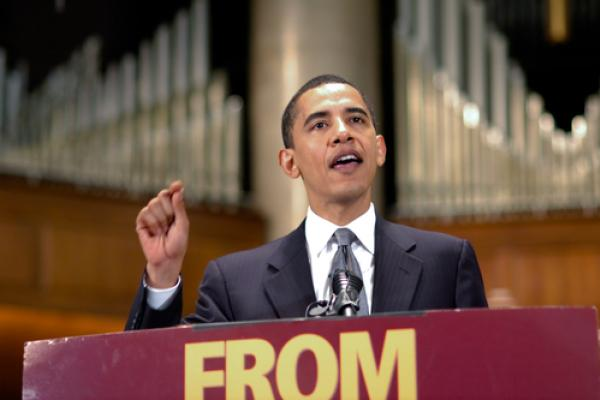
\includegraphics[width=8cm]{P2023.AIBCCSS.Change/change.Obama.jpg}
 
 \end{center}
 
\begin{center}
\tiny
Source of the content: \url{https://sojo.net/articles/transcript-obamas-2006-sojournerscall-renewal-address-faith-and-politics}.
\end{center}
\end{frame}

\begin{frame}
{\centerline{Change as a ``magic'' buzzword (4/6)}}
 
\begin{itemize}
 \item Renewal and change in South Africa:
 \end{itemize} 
\begin{center}
 
\includegraphics[width=8cm]{P2023.AIBCCSS.Change/SouthAfrica.Change.jpg}
 
 \end{center}
 
\begin{center}
\tiny
Source of the content: \url{https://www.youtube.com/watch?v=sg5Wi3BFiWs}.
\end{center}



\end{frame}

\begin{frame}
{\centerline{Change as a ``magic'' buzzword (5/6)}}
 
\begin{itemize}
 \item Rinnovamento Italiano:
 \end{itemize} 
\begin{center}

\includegraphics[width=4cm]{P2023.AIBCCSS.Change/RinnovamentoItaliano.png}
 
 \end{center}
 
\begin{center}
\tiny
Source of the content: \url{https://it.wikipedia.org/wiki/Rinnovamento_Italiano}.
\end{center}



\end{frame}	

\begin{frame}
{\centerline{Change as a ``magic'' buzzword (6/6)}}
 
\begin{itemize}
 \item Il bolscevico -- \textcolor{orange}{Change Italy}:
 \end{itemize} 
\begin{center}
 
\includegraphics[width=4cm]{P2023.AIBCCSS.Change/change.IlBolscevico.jpg}
 
 \end{center}
 
\begin{center}
\tiny
Source of the content: \url{https://www.calameo.com/read/000726878e48538138235}.
\end{center}



\end{frame}




\begin{frame}
{\centerline{Beware of change and renewals!}}

\begin{itemize}
\item Change can be simply used as a buzzword to handle undesired actions
\item Remember also some statements about change:
\begin{itemize}
\item ``If we want that everything remains as it is, we need to change everything,'' Giuseppe Tommasi di Lampedusa in his roman ``The Leopard''
\item ``[the king] has avoided the civil war and has allowed to insert in the tired arteries of the parliamentary constitution the new, impetuous fascist flow, which has emerged from the war and has been exalted by the victory,'' Benito Mussolini in his speech at the Lower Chamber of the Parliament, 1922
\end{itemize} 
\end{itemize} 

\end{frame}

\begin{frame}
{\centerline{The focus of our work}}


\begin{itemize}
\item We have reviewed a few situations where the word ``change'' or his very synonym ``renewal'' could be found
\item We will now pose the attention to a fundamental question:
\begin{itemize}
\item \textcolor{red}{Is change possible?}
\end{itemize} 
\item And we will focus our analysis to a well defined context, the most challenging for changes:
\begin{itemize}
\item Is change possible \textcolor{red}{in development processes}?
\end{itemize} 
\item \textit{which amount to ask}:
\begin{itemize}
\item Is it possible to \textcolor{blue}{change how people use their individual and their collective minds} to develop software?
\end{itemize} 
\item \textit{and also}:
\begin{itemize}
\item Are \textcolor{cyan}{\textbf{cognitive architectures immutable}}?
\end{itemize} 
\end{itemize} 

\end{frame}

\begin{frame}
{\centerline{The experiment of Belyaev (1/3)}}


\begin{itemize}
\item Researcher: Dmitry Belyaev
\item Goal: to bread foxes with the behaviour of friendly dogs
\item Location: Institute of Cytology and Genetics, Siberia
\item Years: 1958 - now
\item Structure
\begin{itemize}
\item Foxes originally bread for fur were tested for friendliness toward the human being
\begin{itemize}
\item just inserting a hand in the cage, nothing more
\end{itemize} 
\item those who were friendly were kept and mated
\item this was repeated for generations after generations
\item the six generation provided a huge surprise
\end{itemize} 

\end{itemize} 

\begin{center}
\tiny
Source of the content: Lyudmila Trut, Lee Alan Dugatkin ``Wild Foxes Can Be Transformed into Pets in a Few Generations,'' Scientific America, May 1, 2017 -- \url{https://www.scientificamerican.com/article/wild-foxes-can-be-transformed-into-pets-in-a-few-generations/}.
\end{center}

\end{frame}


\begin{frame}
{\centerline{The experiment of Belyaev (2/3)}}


\begin{itemize}
\item At the sixth generation foxes appeared that had a very ``dog-like'' behaviour:
\begin{itemize}
\item being very friendly to humans, and seeking their contact,
\item wagging tales,
\item whining and whimpering,
\item licking,
\item recognizing their names.
\end{itemize}  
\end{itemize} 

\begin{center}
 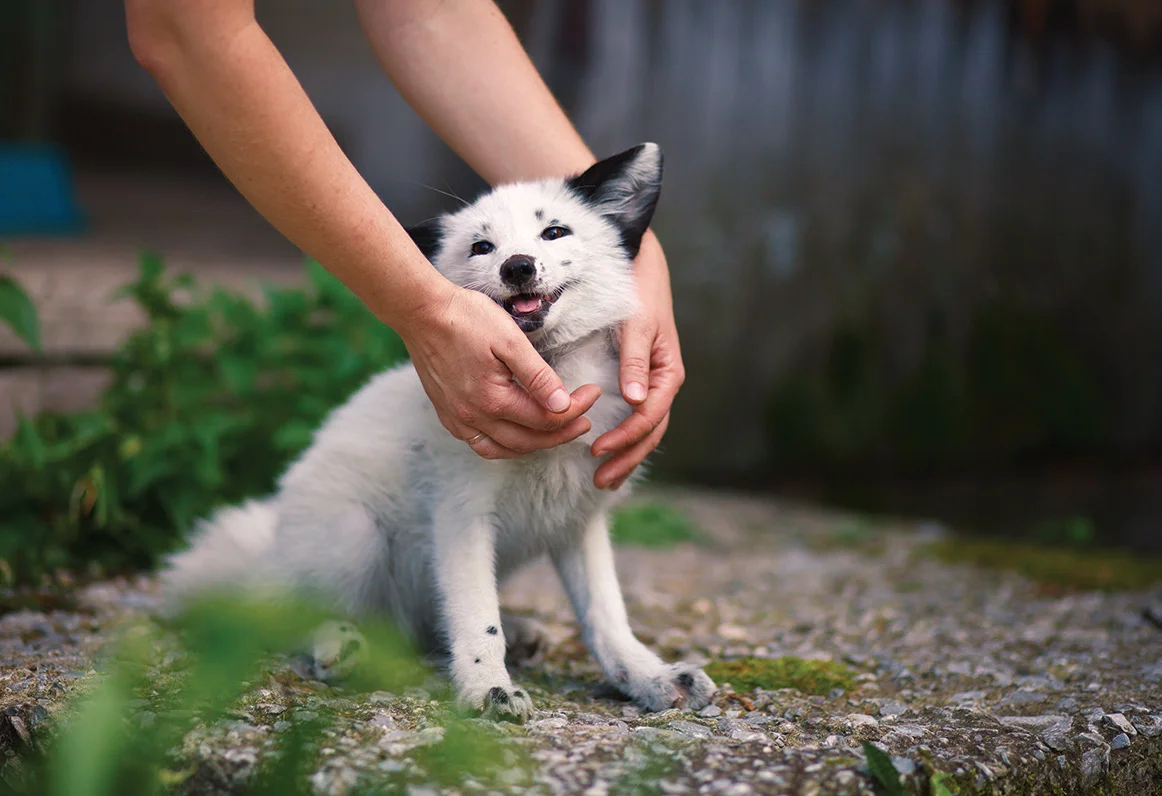
\includegraphics[width=4cm]{P2023.AIBCCSS.Change/tamefoxes.jpg}
 
 \end{center}


\begin{center}
\tiny
Source of the content and of the picture: Lyudmila Trut, Lee Alan Dugatkin ``Wild Foxes Can Be Transformed into Pets in a Few Generations,'' Scientific America, May 1, 2017 -- \url{https://www.scientificamerican.com/article/wild-foxes-can-be-transformed-into-pets-in-a-few-generations/}.
\end{center}

\end{frame}


\begin{frame}
{\centerline{The experiment of Belyaev (3/3)}}


\begin{itemize}
\item and this is not the end:
\begin{itemize}
\item  the percentage of tame foxes increased generation after generation
\item after a while also the morphological features of the tame foxes changed:
\begin{itemize}
\item floppy ears,
\item black and white colours,
\item bushier tales, and once
\item barked!
\end{itemize}
\end{itemize} 
 


\end{itemize} 

\begin{center}
\tiny
Source of the content: Lyudmila Trut, Lee Alan Dugatkin ``Wild Foxes Can Be Transformed into Pets in a Few Generations,'' Scientific America, May 1, 2017 -- \url{https://www.scientificamerican.com/article/wild-foxes-can-be-transformed-into-pets-in-a-few-generations/}.
\end{center}

\end{frame}




\begin{frame}
{\centerline{Toward Cognitive Restructuring}}


\begin{itemize}
\item How can we translate this into software engineering
\item Psychology has focused on changing the behaviour of people for decades
\item We have found that an approach for treating people could be effective also in enacting positive changes of processes
\begin{itemize}
\item especially those related to agile methods, methods emphasizing cognitive architectures and collective intelligence
\end{itemize} 
\item Cognitive restructuring has been advocated as an approach
\item Cognitive restructuring is strongly related to the dual impulsive/reflective model
\end{itemize} 

\begin{center}
\tiny
Source of the content: \url{https://en.wikipedia.org/wiki/Cognitive_restructuring}.
\end{center}

\end{frame}

\begin{frame}
{\centerline{Cognitive Behavioural Therapy (1/2)}}

\begin{itemize}
\item Cognitive restructuring is at the root of \textcolor{red}{Cognitive Behavioural Therapy}
\end{itemize} 

\begin{center}
 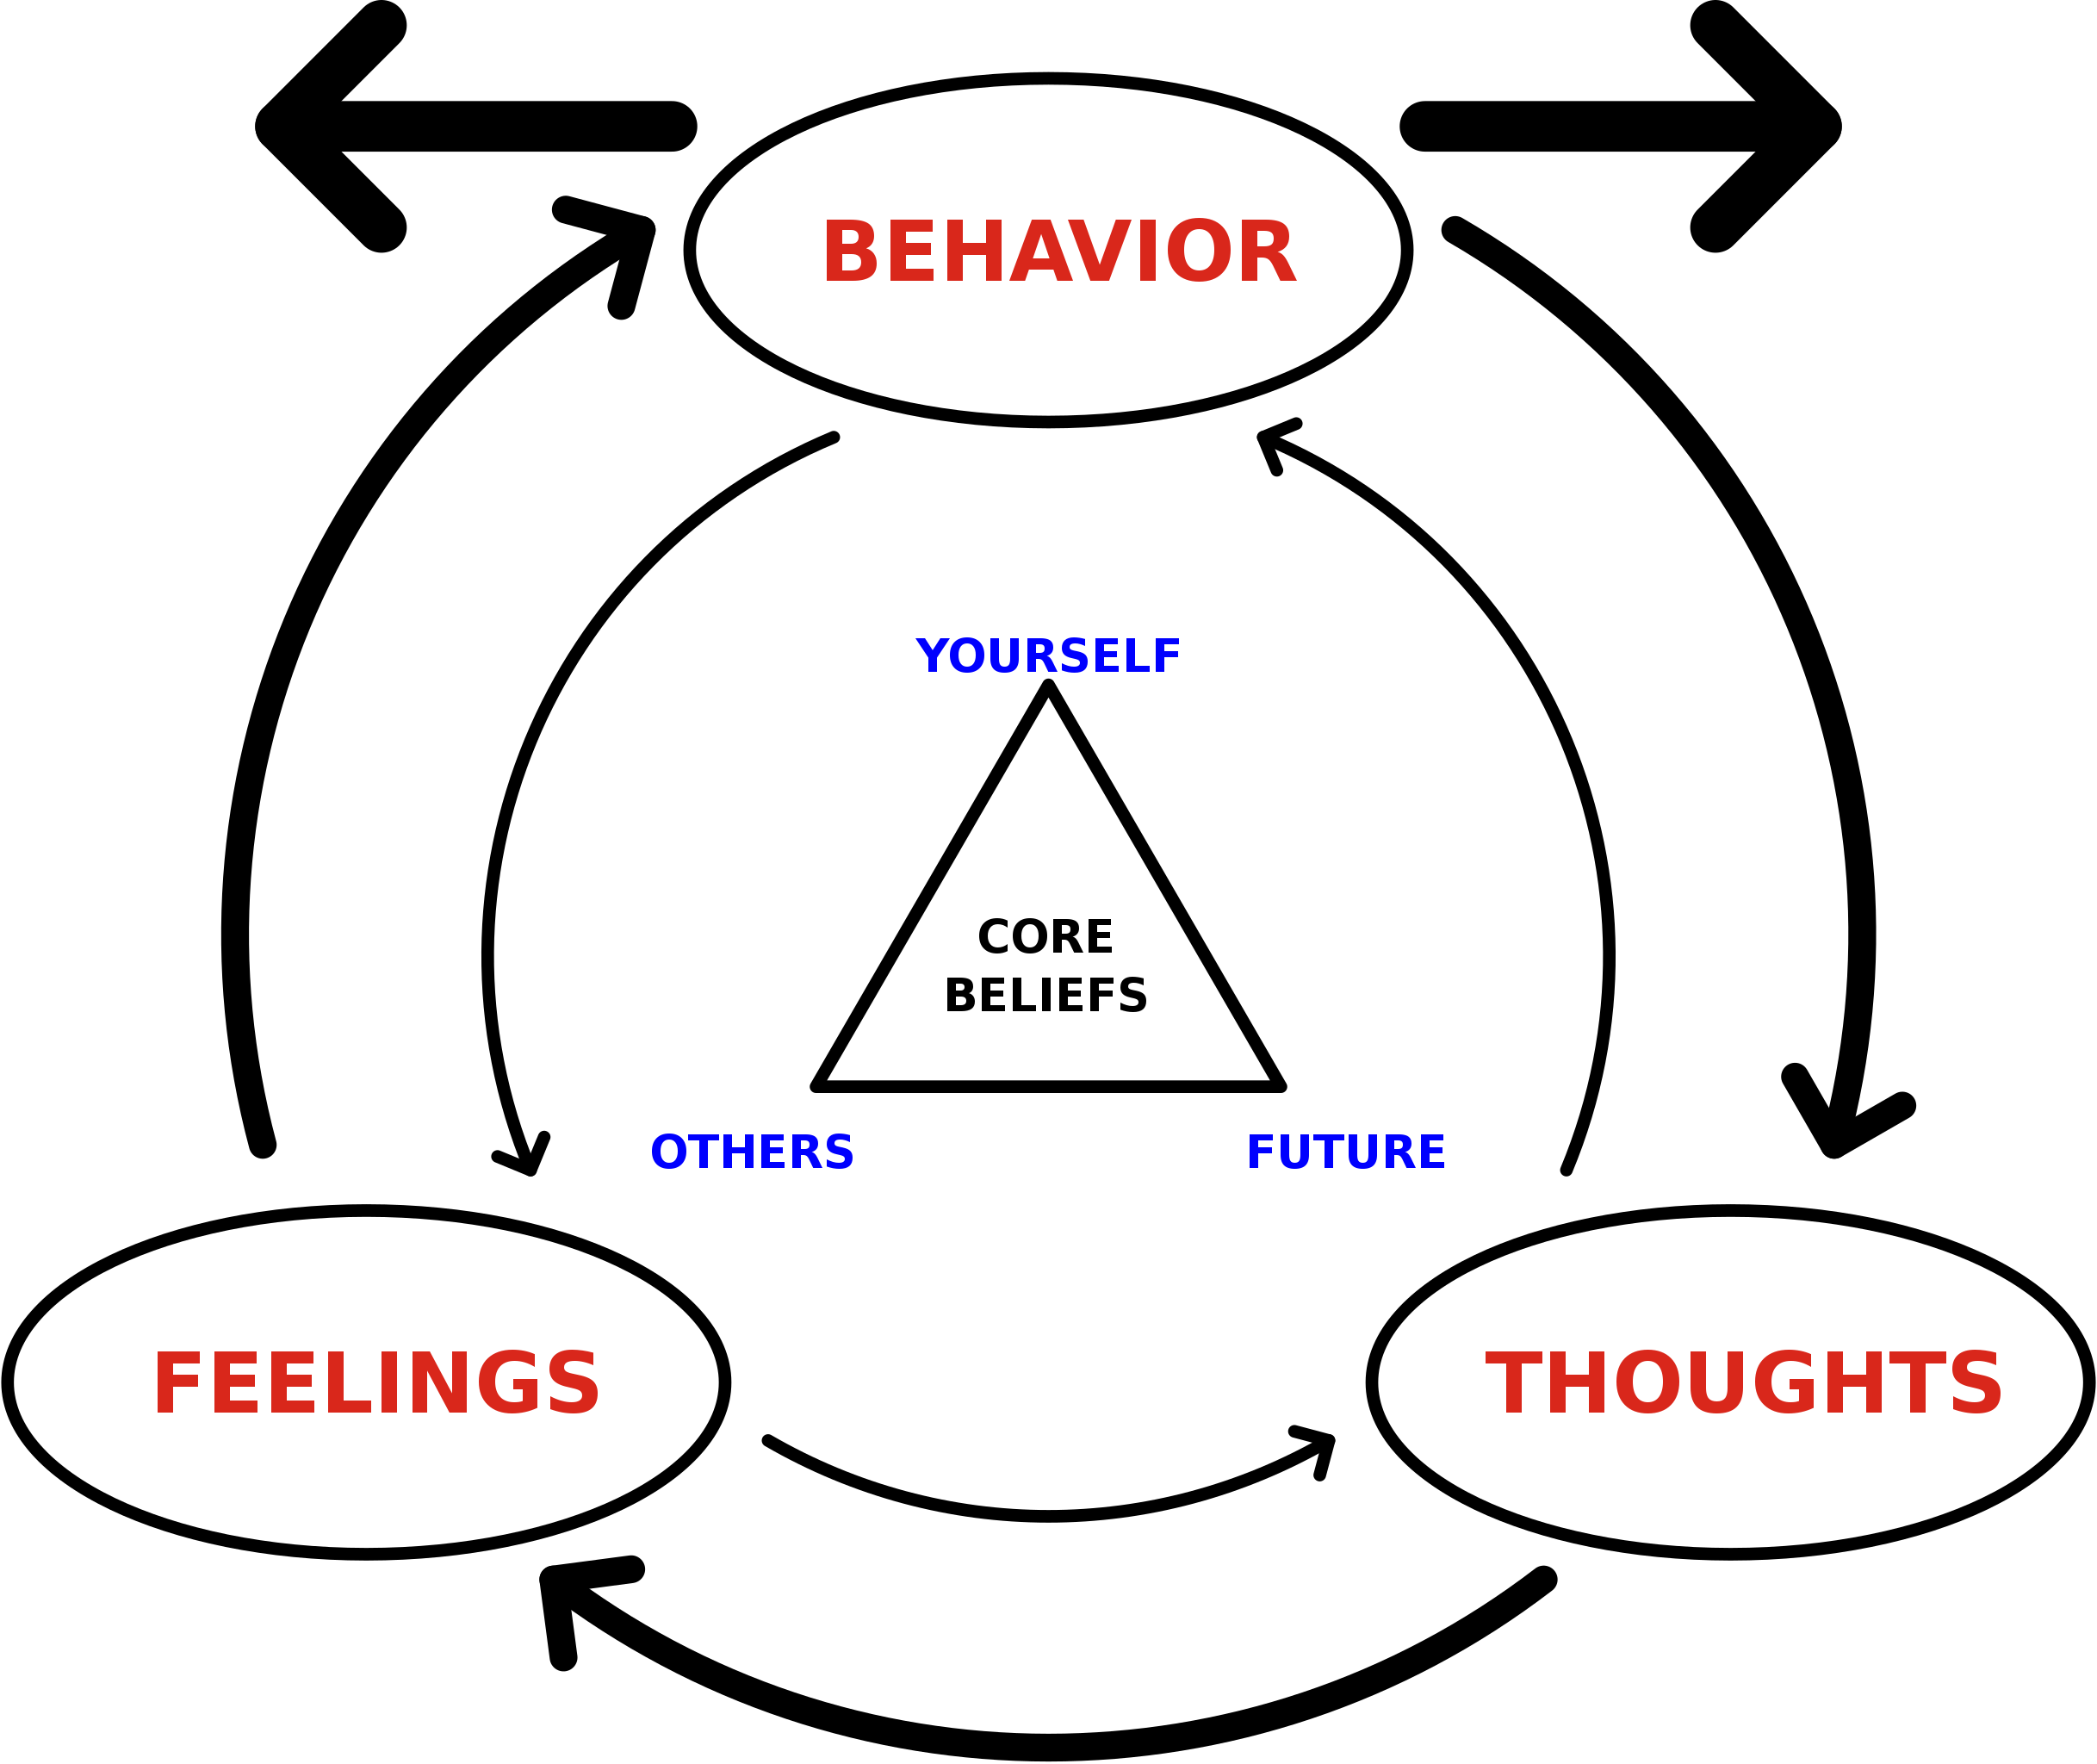
\includegraphics[width=6cm]{P2023.AIBCCSS.Change/Cognitive_behavioral_therapy.png}
 
 \end{center}
 
 \begin{center}
\tiny
Source of the content: \url{https://en.wikipedia.org/wiki/Cognitive_behavioral_therapy}.
\end{center}


\end{frame}

\begin{frame}
{\centerline{Cognitive Behavioural Therapy (2/2)}}

\begin{itemize}
\item Centered on removing altered beliefs on the reality
\item It is a talk therapy
\item Based on the following steps (copied verbatim from wikipedia):
\begin{itemize}
\item Assessment or psychological assessment;
\item Reconceptualization;
\item Skills acquisition;
\item Skills consolidation and application training;
\item Generalization and maintenance;
\item Post-treatment assessment follow-up.
\end{itemize} 
\end{itemize} 

\begin{center}
\tiny
Source of the content: \url{https://en.wikipedia.org/wiki/Cognitive_behavioral_therapy}.
\end{center}

\end{frame}

\begin{frame}
{\centerline{Cognitive Restructuring (1/2)}}

\begin{itemize}
\item Cognitive restructuring focuses on eliminating problematic ``\textcolor{red}{automatic thoughts},'' which we can consider kind of \textcolor{cyan}{heuristics}
\item We can perceive here the presence of the dual model \textcolor{orange}{Impulsive/Reflective}
\item Four steps in cognitive restructuring
\item \textit{(Again copying almost verbatim from wikipedia)}
\begin{itemize}
\item Identification of automatic thoughts
\item Identification of the cognitive distortions in automatic thoughts
\item Rational disputation of automatic thoughts with the Socratic method
\item Development of a rational rebuttal to the automatic thoughts.
\end{itemize} 
\end{itemize} 

\begin{center}
\tiny
Source of the content: \url{https://en.wikipedia.org/wiki/Cognitive_restructuring}.
\end{center}

\end{frame}

\begin{frame}
{\centerline{Cognitive Restructuring (2/2)}}

\begin{itemize}
\item There is a taxonomy of automatic thoughts
\item \textit{(Again copying almost verbatim from wikipedia)}
\begin{itemize}
\item Self-evaluated thoughts
\item Thoughts about the evaluations of others
\item Evaluative thoughts about the other person with whom they are interacting
\item Thoughts about coping strategies and behavioral plans
\item Thoughts of avoidance
\item Others
\end{itemize} 
\item Thoughts may be elicited and recorded via \textcolor{red}{Though Records}
\end{itemize} 

\begin{center}
\tiny
Source of the content: \url{https://en.wikipedia.org/wiki/Cognitive_restructuring}.
\end{center}

\end{frame}

\begin{frame}
{\centerline{Example of ``Thought Record'' in CBT}}

\begin{center}
 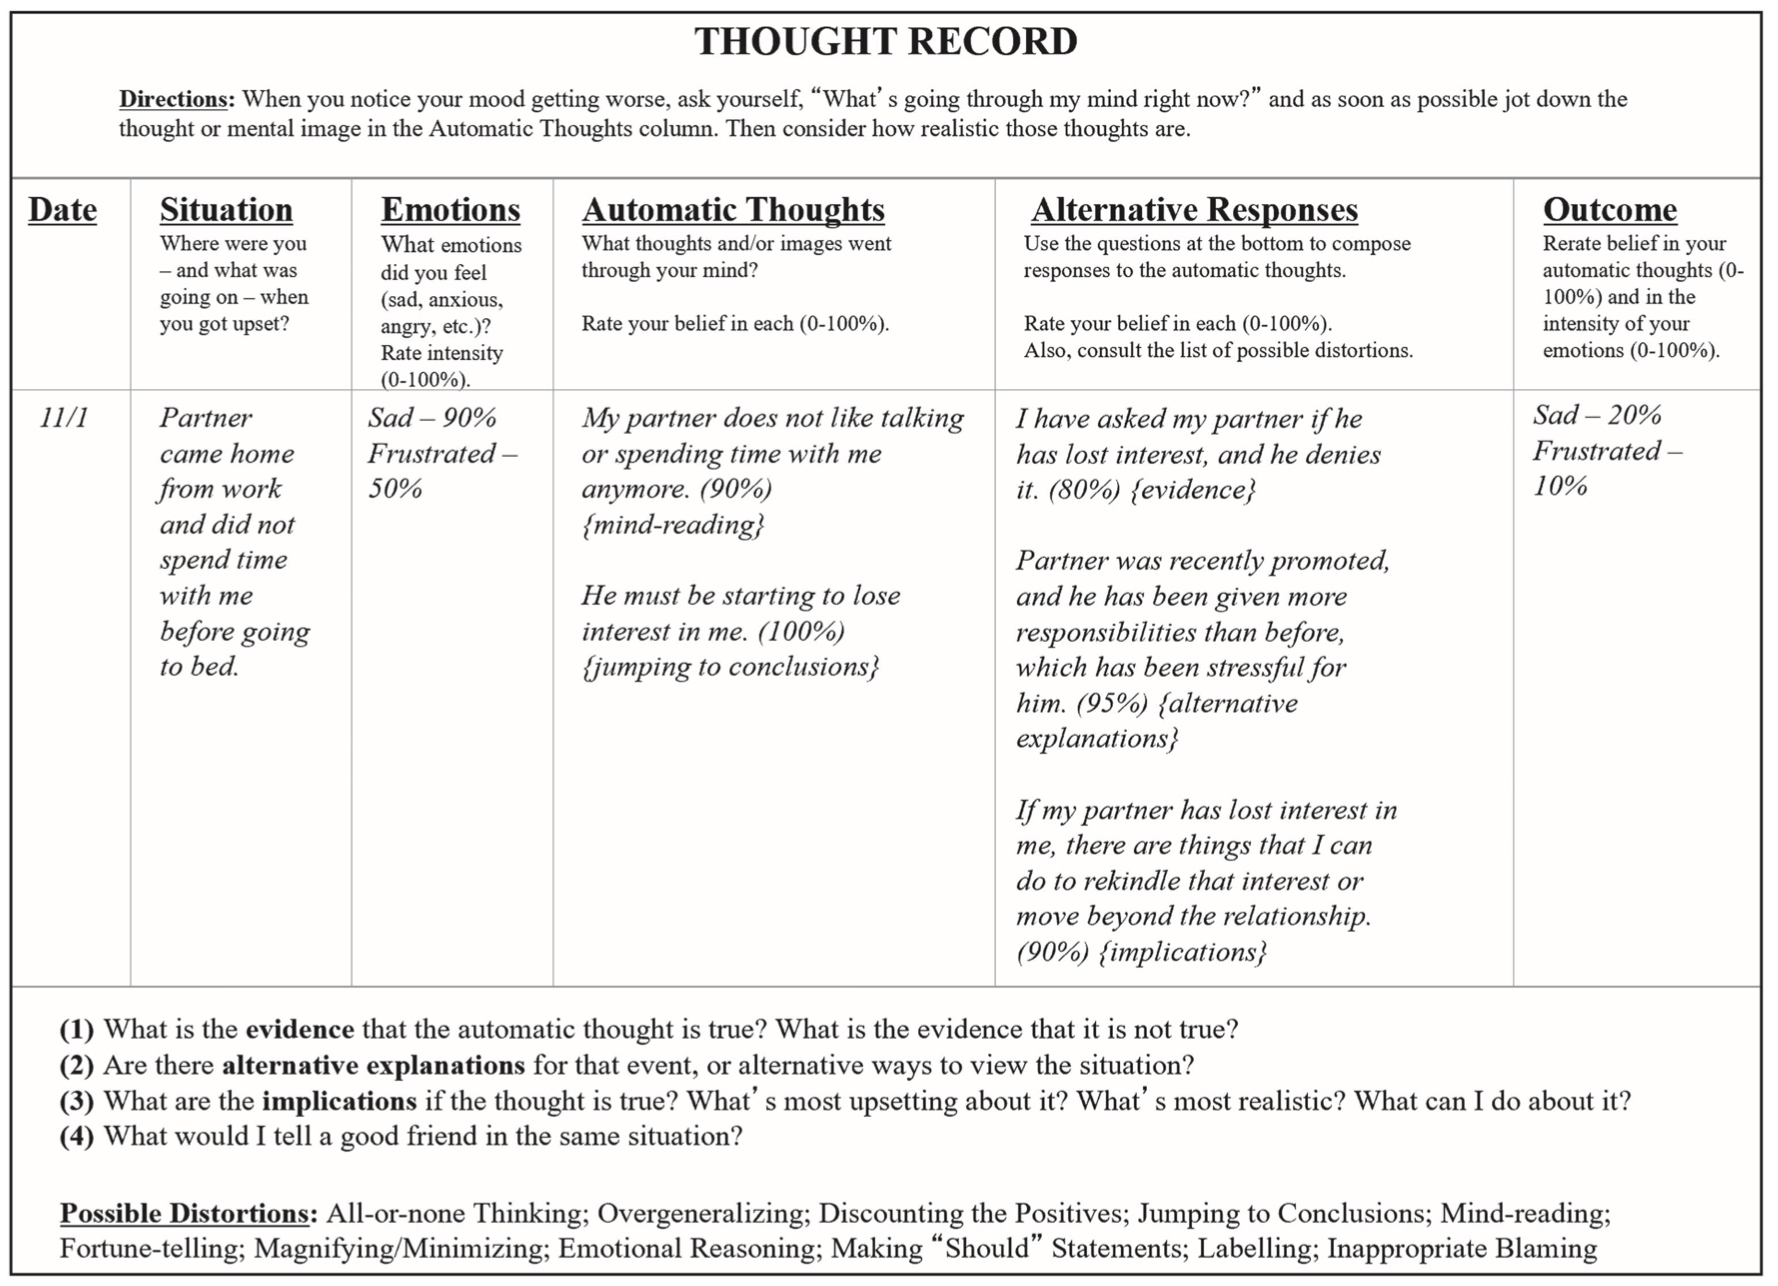
\includegraphics[width=9cm]{P2023.AIBCCSS.Change/thoughtRecord.jpg}
 
 \end{center}
 
 \begin{center}
\tiny
Source of the content: Ezawa ID, Hollon SD. Cognitive restructuring and psychotherapy outcome: A meta-analytic review. Psychotherapy (Chic). 2023 Mar 13, Fig. 1.
\end{center}


\end{frame}

\begin{frame}
{\centerline{Effectiveness of Cognitive Restructuring}}

\begin{center}
 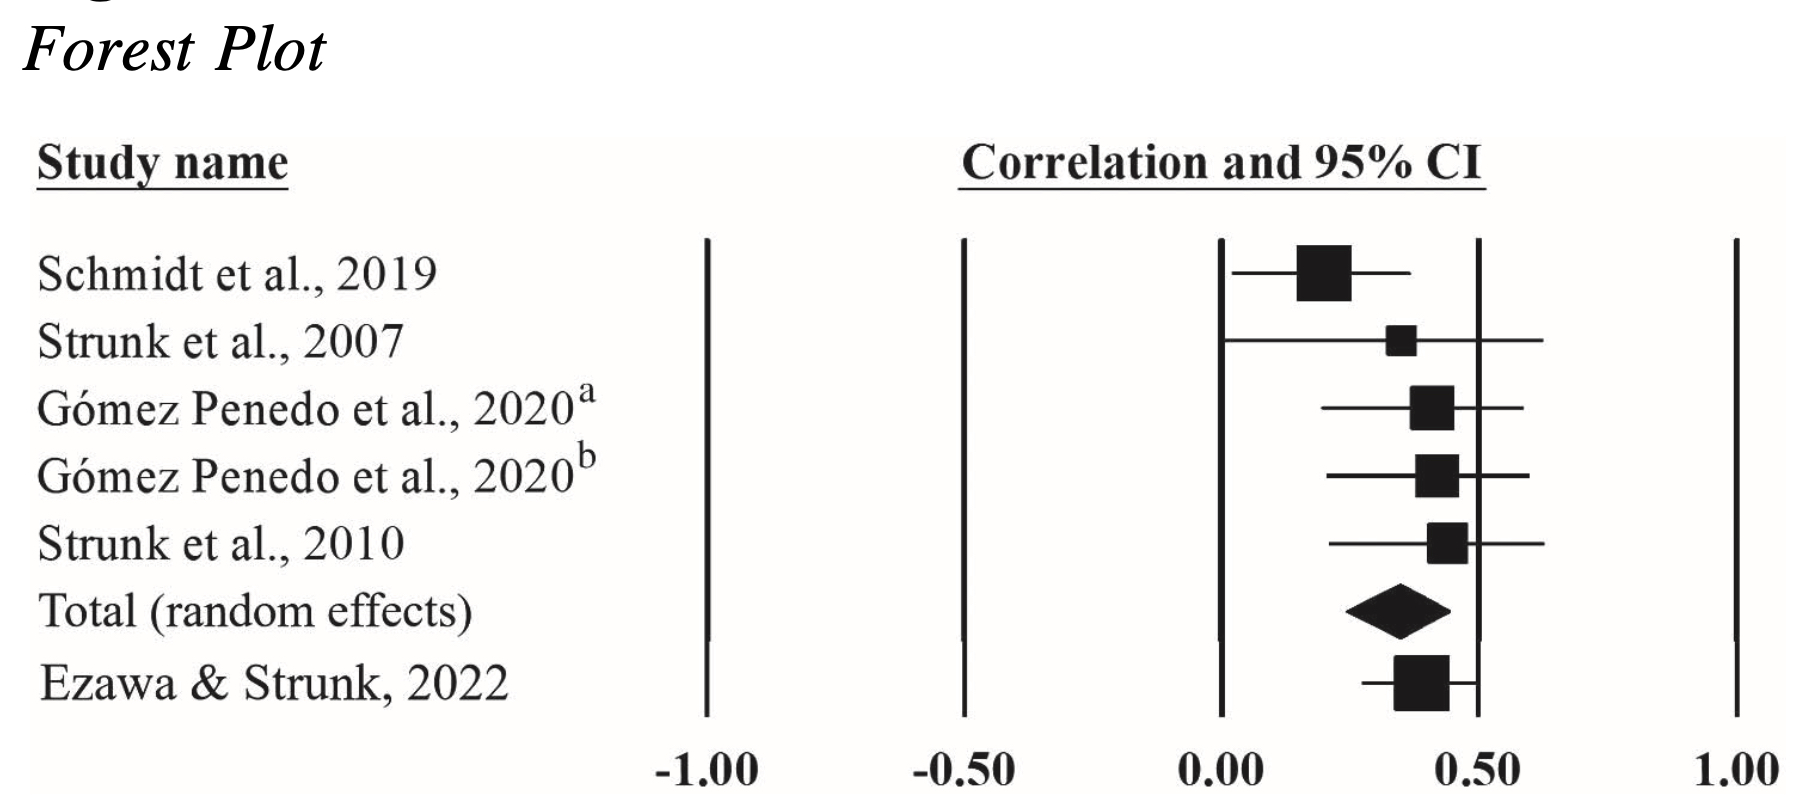
\includegraphics[width=12cm]{P2023.AIBCCSS.Change/effectivenessCR.jpg}
 
 \end{center}
 
 \begin{center}
\tiny
Source of the content: Ezawa ID, Hollon SD. Cognitive restructuring and psychotherapy outcome: A meta-analytic review. Psychotherapy (Chic). 2023 Mar 13, Fig. 2.
\end{center}


\end{frame}

\begin{frame}
{\centerline{Applying cognitive restructuring}}

\begin{itemize}
\item Cognitive restructuring is most effective if the target of it understand its cognitive model:
\begin{itemize}
\item Frontal instruction
\item Active modeling
\item Role playing with feedback
\item Supervision
\end{itemize} 
\item Start with negative automatic thoughts, especially in specific situations
\item Then, extend to core beliefs
\end{itemize} 


\begin{center}
\tiny
Source of the content: \url{https://en.wikipedia.org/wiki/Cognitive_restructuring}.
\end{center}

\end{frame}


\begin{frame}
{\centerline{FYI -- Specific practices related to CR}}

\begin{itemize}
\item Helping identifying, challenging, and correcting wrong negative thoughts, and thus:
\begin{itemize}
\item Treating several disorders, including depression, anxiety, social anxiety, obsessive–compulsive disorder, and posttraumatic stress disorder.
\item Applying it to foster cognitive change and subsequent symptom improvement
\end{itemize} 
\item Problems of biases with marginalized populations.
\item Recall that the goal is \textcolor{red}{not to minimize existing threats} but rather \textcolor{cyan}{\bf to get an accurate sense of what threats might be}.
\end{itemize} 

\begin{center}
\tiny
Source of the content: \url{https://en.wikipedia.org/wiki/Cognitive_restructuring}.
\end{center}

\end{frame}




\begin{frame}{\centerline{XP and Cognitive Restructuring (1/3)}}

\begin{itemize}
\item  Extreme Programming (XP) is one of the \textcolor{cyan}{most relevant agile methods}
\item  We can clearly see a neat application of CR and CBT in its structure:
\begin{itemize}
\item XP is structured in \textcolor{red}{Values}, \textcolor{blue}{Drivers}, and \textcolor{orange}{Practices}
\end{itemize}
\end{itemize}


\begin{columns}
\begin{column}{0.5\textwidth}
\begin{itemize}
\item 4 \textcolor{red}{Values}:
\begin{itemize}
\item  Simplicity
\item Communication
\item Feedback
\item Courage
\end{itemize}
\end{itemize}

\end{column}

\begin{column}{0.5\textwidth} 
\begin{itemize}
\item 3 \textcolor{blue}{Drivers}:
\begin{itemize}
\item  Focus on value
\item  Constant flow of activities
\item  No defects
\end{itemize}
\end{itemize}

\end{column}

\end{columns}


\end{frame}
%=============================================

%---------------------------------------------
\begin{frame}{\centerline{ XP and Cognitive Restructuring (2/3)}}
% Nr:33

\begin{center}
 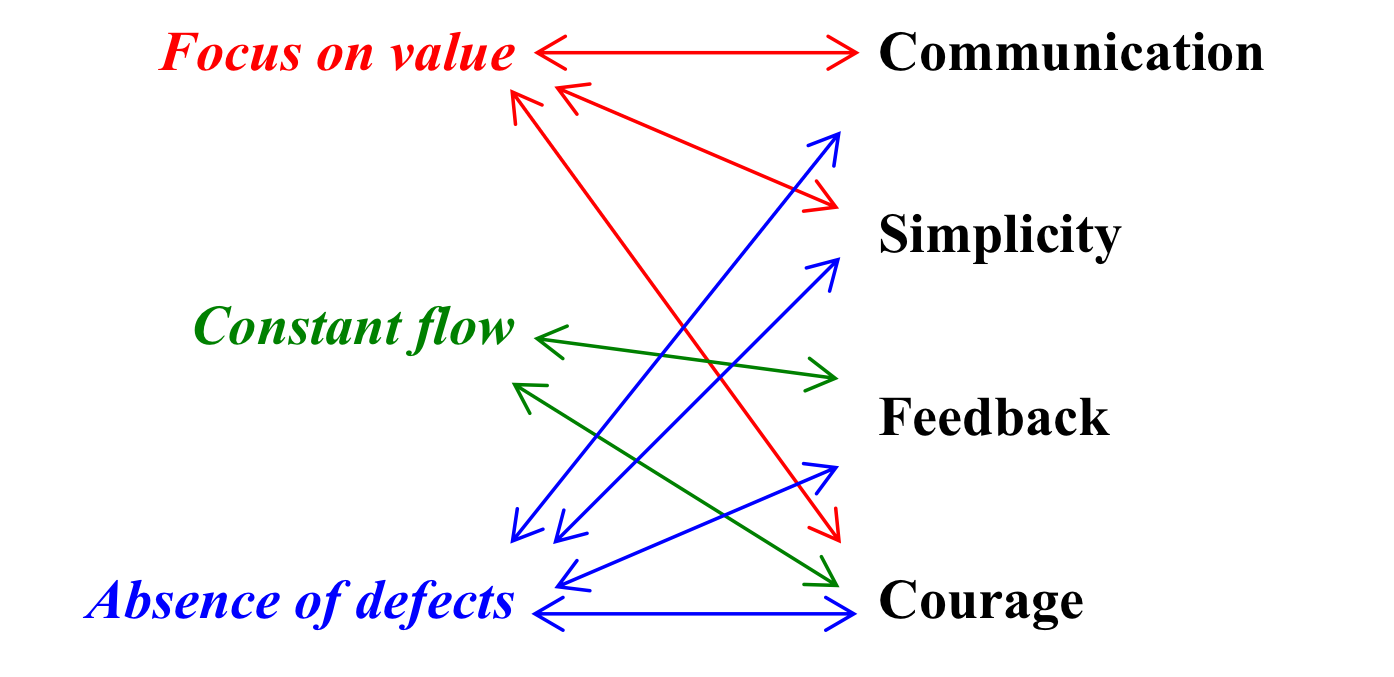
\includegraphics[width=10cm]{P2023.AIBCCSS.Change/valuesDrivers.XP.png}
 
 \end{center}

\end{frame}
%=============================================

%---------------------------------------------
\begin{frame}{\centerline{XP and Cognitive Restructuring (3/3)}}
% Nr:34

\begin{center}
\textcolor{orange}{\bf Practices:}
\end{center}

\begin{columns}
\begin{column}{0.5\textwidth}

\begin{itemize}
\item  Planning game
\item Short releases
\item Metaphor
\item  Simple design
\item Test-driven development
\item  Refactoring
\end{itemize}

\end{column}
\begin{column}{0.5\textwidth} 

\begin{itemize}
\item  Pair programming
\item Collective code ownership
\item Continuous integration
\item 40 hours working week
\item On-site customer
\item Coding standards
\end{itemize}
\end{column}

\end{columns}

\end{frame}

\begin{frame}
{\centerline{Extreme Programming -- \textcolor{red}{Embrace Change}}}

\begin{center}
 \includegraphics[width=5cm]{P2023.AIBCCSS.Change/extremeProgrammingCover.jpg}
 
 \end{center}
 
 \begin{center}
\tiny
Source of the picture: Front cover of: Beck, K. (1999). Extreme Programming Explained: Embrace Change. Addison-Wesley Publishing Company.
\end{center}


\end{frame}


\begin{frame}
{\centerline{Questions?}}

\vspace{1cm}
\begin{center}
    \LARGE{End of lecture eight.}
\end{center}

\end{frame}


\end{document}
